\documentclass[a4paper,oneside,12pt]{article}
\usepackage[slovene]{babel}
\usepackage[utf8]{inputenc}
\usepackage[T1]{fontenc}
\usepackage[reqno]{amsmath}
\usepackage{amssymb}
\usepackage{amsfonts}
\usepackage{tabularx}
\usepackage{lmodern}
\usepackage{graphicx}
\usepackage{geometry}
\usepackage{xcolor}

\newtheorem{definicija}{Definicija}


\begin{document}
	
\begin{titlepage}
	
	\centering
	
	\textsc{\large Univerza v Ljubljani}\\[0.3cm]
	
	{\Large Fakulteta za matematiko in fiziko}\\[3cm]
	
	{\Huge Poročilo}\\[0.3cm]
	
	\textsc{\Huge Naključni sprehodi po mrežah}\\[2cm]
	
    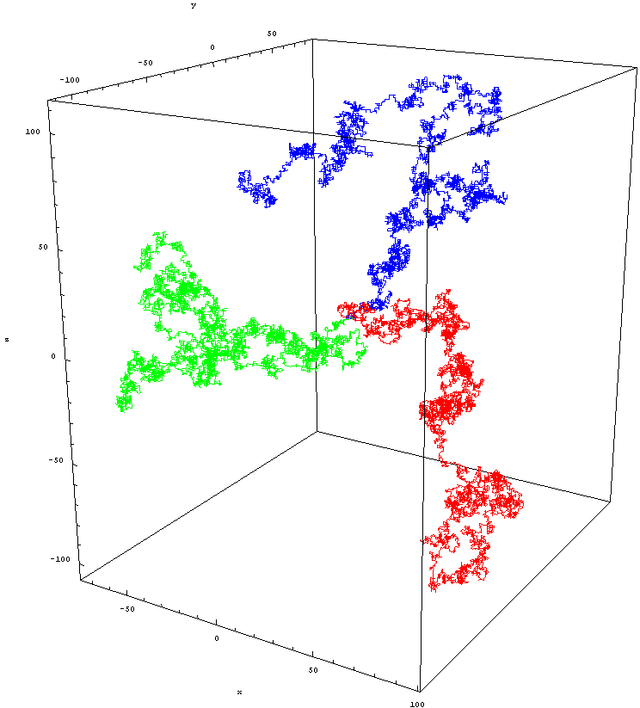
\includegraphics[width=0.4\textwidth]{random3D}\\[2.5cm]

	\begin{minipage}{0.45\linewidth}
		\begin{flushleft}
			\large
			\textit{Avtorja:}\\
			Ian Spiller \\
			Šida Talović 
		\end{flushleft}
    \end{minipage}
~
    \begin{minipage}{0.45\linewidth}
		\begin{flushright}
			\large
			\textit{Mentorja:}\\
			prof. dr. Sergio Cabello \\
			doc. dr. Janoš Vidali
		\end{flushright}		
	\end{minipage}\\[1.5cm]  

\vfill\vfill

{\large{Ljubljana, \today}} 

\vfill 

\end{titlepage}	
\newpage
\tableofcontents
\newpage	

\section{Uvod}
Pri projektu sva opazovala lastnosti diskretnih naključnih sprehodov po $\mathbb{Z}^n$,\\ $n = 1, 2, 3, 5, 10, 50$, potem pa to posplošila na $n$ $\rightarrow$ $\infty$. V poročilu najprej sledi opis problema potem pa še potek dela, 
razmisleki ter ugotovitve. Reševanja problema sva se lotila s programiranjem v Pythonu, kjer sva napisala program naključnega sprehoda, ki nama v \texttt{.xlsx} datoteki vrne izračune ter grafe porazdelitev. 

\section{Reševanje problema}

\subsection{Navodilo}
Razmislite o neskončni d-dimenzionalni mreži. Oglišča so točke koordinat celih števil in dve oglišči sta povezani, ko se v posamezni koordinati razlikujeta za eno vrednost. 
Začetek je poljubno izbran: na vsakem koraku naključno izberite soseda trenutnega oglišča in se premaknete tja. Eksperimentalno analizirajte lastnosti tega naključnega sprehoda. 
Kako pogosto se vračate na izvor? Kakšna je porazdelitev razdalje od izhodišča? Kako so lastnosti odvisne od dimenzije d? Prepričajte se, da uporabite nekaj dobrih generatorjev naključnih številk/bitov.


\begin{definicija} Naključni sprehod po mreži s celoštevilskimi oglišči in dimenzijo n je naključni proces, pri katerem se na vsakem koraku naključno premaknemo na eno od točk oddaljenih za eno enoto. Naključni sprehod je simetričen, če je verjetnost premika v vsako smer enaka, sicer je nesimteričen.
\end{definicija}

\subsection{Potek dela}
Problema sva se lotila tako, da sva preučevane lastnosti preverila za 1-, 2-, 3-, 5-, 10- in 50-dimenzionalne mreže, potem pa te ugotovitve poskušala posplošiti na višje dimenzije. 
Opazovala sva slučajne sprehode z 200, 500 in 1000 slučajnimi koraki ter vsak slučajni sprehod ponovila 40-krat in 80-krat ter primerjala rezultate. \\


 \subsection{Koda v Pythonu}

 Program kot vhodne podatke sprejme seznam v katerem navedemo za katere dimenzije želimo dobiti podatke,
 število korakov slučajnega sprehoda ter kolikokrat naj se ponovi slučajni sprehod za določeno dimenzijo.
 V programu potem uporabimo funkcijo \texttt{enake\_ver}, ki naredi seznam seznamov, kjer vsak podseznam predstavlja obiskane točke slučajnega sprehoda.
 Funkcija slovar nato vzame ta seznam in generira nov slovar, kjer so ključi točke, vrednosti pa oddaljenost od izhodišča, kolikokrat je slučajni sprehod prišel v to točko in ob katerem času. Program se nato za vsako izbrano dimenzijo ponovi tolikokrat kot smo določili in v vsaki ponovitvi izračuna kolikokrat sta se srečala dva neodvisna slučajna sprehoda, ali se je slučajni sprehod vrnil v izhodišče, povprečno oddaljenost, zapomni si najdaljšo oddaljenost od izhodišča, ki se je pojavila v tej ponovitvi slučajnega sprehoda in naredi slovar, v katerem so ključi oddaljenosti od izhodišča, vrednosti pa kolikokrat se je ta oddaljenost pojavila v vseh ponovitvah do sedaj. Ko program opravi vse ponovitve izračuna, vsa željena 
 povprečja poleg tega pa v slovarju z razdaljami izračuna, kolikokrat se je v povprečju pojavila posamezna razdalja in naredi seznam v katerem se vsaka razdalja pojavi tolikokrat kot se je pojavila v povprečju.
 To nam omogoči, da dobimo lepši graf porazdelitve oddaljenosti od izhodišča. Program nam nato kot rezultat naredi \texttt{.xlsx} dokument, v katerem dobimo grafe porazdelitev oddaljenosti od izhodišča in tabelo v kateri so naslednje vrednosti:
\begin{itemize}
     \item povprečna oddaljenost od izhodišča (program vzame povprečno oddaljenost od izhodišča v vsakem sprehodu in izračuna povprečje),
     \item povprečna največja oddaljenost od izhodišča (program vzame najdaljšo razdaljo v vsaki ponovitvi in izračuna povprečje),
     \item najdaljša razdalja (program vrne najdaljšo razdaljo, ki jo je zabeležil v vsah ponovitvah slučajnega sprehoda),
     \item število vrnitev v izhodišče (program vrne v koliko ponovitvah slučajnega sprehoda smo se vrnili v izhodišče),
     \item povprečno število srečanj (program vrne kolikokrat sta se v povprečju srečala dva neodvisna slučajna sprehoda, torej program dobi seznam
     v katerem so števila srečanj za posamezno dimenzijo in izračuna povprečje),
     \item v koliko ponovitvah se srečata (program nam pove v koliko ponovitvah sta se srečala neodvisna slučajna sprehoda, ni pa pomembno kolikokrat sta se 
     srečala v posamezni ponovitvi).
\end{itemize}
\bigskip

\section{Rezultati in ugotovitve}
\subsection{Izračuni}

Ko zaženenemo kodo iz prejšnjega podpoglavja, dobimo \texttt{.xlsx} datoteko z izračuni ter grafe porazdelitev. Program sva zagnala za veliko različnih vrednosti ter si pogledala, kako se vrednosti spreminjajo s številom korakov (100, 200, 500, 1000) slučajnega sprehoda in z različnim številom ponovitev (40, 80, 200) le tega. 
Ugotovila sva določene trende povezane z obema parametroma in se odločila, 
da bova prikazala podatke za 200 korakov in 40 ponovitev, za 500 korakov in 40 ponovitev in na koncu še za 500 korakov in 80 ponovitev.
\bigskip

\begin{center}
\begin{tabular}{|c| c c c c c c|} 
\hline
dimenzija & 1 & 2 & 3 & 5 & 10 & 50 \\ [0.5ex] 
\hline \hline 
povprečna oddaljenost od izhodišča & 6.4 & 10.7 & 12.4 & 16.5 & 22.3 & 49 \\ [0.5ex] 
\hline
povprečna najdaljša oddaljenost & 15.9 & 21.4 & 24.1 & 29.4 & 36.4 & 78.4  \\ [0.5ex] 
\hline
najdaljša razdalja & 34 & 37 & 42 & 50 & 54 & 97 \\ [0.5ex] 
\hline
število vrnitev v izhodišče & 39 & 26 & 7 & 5 & 1 & 0 \\ [0.5ex] 
\hline
povprečno število srečanj & 15.2 & 1.4 & 0.35 & 0.25 & 0.02 & 0 \\ [0.5ex] 
\hline
v koliko ponovitvah se srečata & 37 & 25 & 7 & 9 & 1 & 0 \\ [0.5ex] 
\hline
\end{tabular}
\end{center}
\bigskip
Pri zgornjih podatkih za oddaljenost od izhodišča dobimo še naslednje grafe porazdelitev:

\begin{figure}[h]
    \centering
    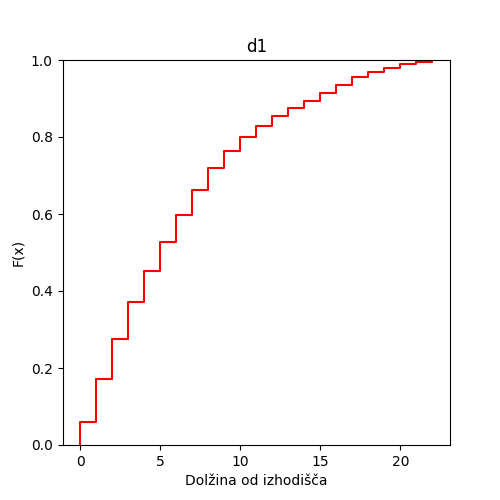
\includegraphics[width=0.25\textwidth]{graf1-1}
    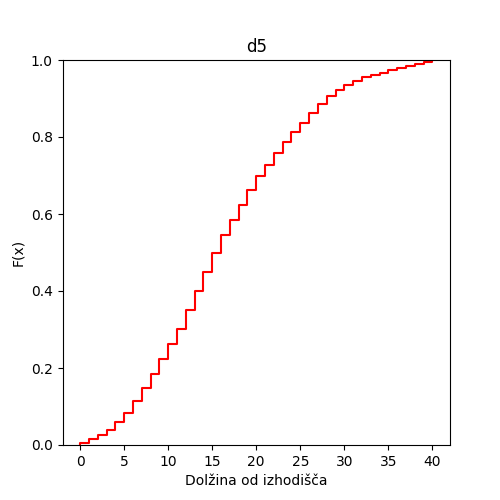
\includegraphics[width=0.25\textwidth]{graf5-1}  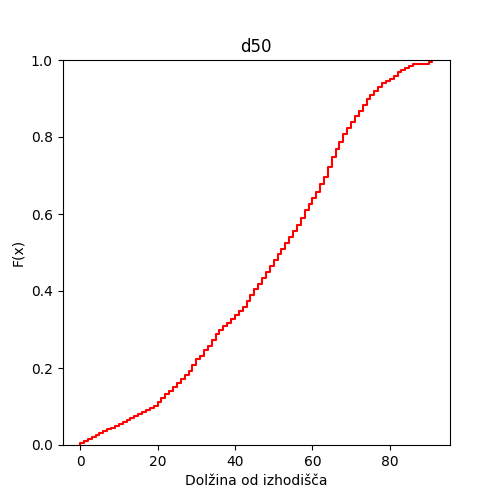
\includegraphics[width=0.25\textwidth]{graf50-1}
    \caption{Grafi porazdelitev v različnih dimenzijah}
\end{figure}
\bigskip
Podobno generirava podatke za 40 ponovitev slučajnega sprehoda s 500 koraki. Dobimo naslednjo tabelo: 

\begin{center}
\begin{tabular}{|c| c c c c c c|} 
\hline
dimenzija & 1 & 2 & 3 & 5 & 10 & 50 \\ [0.5ex] 
\hline \hline 
povprečna oddaljenost od izhodišča & 13.3 & 17.3 & 21.9 & 28.6 & 35.7 & 81.4 \\ [0.5ex] 
\hline
povprečna najdaljša oddaljenost & 30 & 34 & 40.4 & 50.7 & 60.2 & 128.6  \\ [0.5ex] 
\hline
najdaljša razdalja & 59 & 63 & 70 & 95 & 86 & 157 \\ [0.5ex] 
\hline
število vrnitev v izhodišče & 39 & 24 & 15 & 3 & 3 & 2 \\ [0.5ex] 
\hline
povprečno število srečanj & 28.18 & 2.08 & 0.46 & 0.2 & 0.05 & 0.02 \\ [0.5ex] 
\hline
v koliko ponovitvah se srečata & 40 & 30 & 13 & 7 & 2 & 1 \\ [0.5ex] 
\hline
\end{tabular}
\end{center}
\bigskip 
V naslednji tabeli so še podatki za 80 ponovitev slučajnega sprehoda s 500 koraki.

\begin{center}
\begin{tabular}{|c| c c c c c c|} 
\hline
dimenzija & 1 & 2 & 3 & 5 & 10 & 50 \\ [0.5ex] 
\hline \hline 
povprečna oddaljenost od izhodišča & 12 & 15.8 & 21.2 & 27.6 & 37.3 & 80.2 \\ [0.5ex] 
\hline
povprečna najdaljša oddaljenost & 27.2 & 34.5 & 40.6 & 47.8 & 62.6 & 126.5  \\ [0.5ex] 
\hline
najdaljša razdalja & 60 & 79 & 81 & 83 & 101 & 162 \\ [0.5ex] 
\hline
število vrnitev v izhodišče & 74 & 53 & 18 & 11 & 6 & 0 \\ [0.5ex] 
\hline
povprečno število srečanj & 22.08 & 2.16 & 0.36 & 0.11 & 0.05 & 0.01 \\ [0.5ex] 
\hline
v koliko ponovitvah se srečata & 73 & 52 & 19 & 8 & 4 & 1 \\ [0.5ex] 
\hline
\end{tabular}
\end{center}

\subsection{Ugotovitve}
Kot sva zgoraj že omenila sva naredila izračune za različne vrednosti števila korakov in ponovitev slučajnega sprehoda. Pri izbiri vrednosti za ponovitve slučajnega sprehoda sva večkrat generirala podatke za iste parametre in gledala odstopanja glede na to, koliko ponovitev sva naredila. Pri tistih izračunih, kjer sva računala pričakovane vrednosti, bi to lahko verjetno boljše preverila, če bi izračunala še standardni odklon. Vseeno pa se nama je zdelo, da že pri 40 ponovitvah dobiva dovolj dobre podatke za analizo. Pri številu korakov sva pogledala vrednosti 100, 200, 500 in 1000. V primeru 50 dimenzij se nama je zdela nekoliko nizka vrednost 100 korakov, zato sva jo izključila, medtem ko je vrednost 1000 pokazala podobne rezultate kot 500 in se nama ni zdelo smiselno uporabiti zaradi časovne zahtevnosti. Za analizo podatkov pri $1, 2, 3 , 5, 10$ in $50$ dimenzijah sva se odločila, ker se nama je zdelo, da bova na nižjih dimenzijah opazila določene trende in potem
sva to želela potrditi tudi za višje dimenzije. Pogledala sva tudi dimenzije 7, 25 in 100, da slučajno tam ne bi prišlo do kakšnih posebnosti, ampak se je vse ujemalo s pričakovanji. \\
Pri analizi podatkov sva opazila, da povprečna oddaljenost točk, povprečna najdaljša oddaljenost in najdaljša zabeležena razdalja v vseh ponovitvah narašča z dimenzijo in številom korakov slučajnega sprehoda. \\
To sva tudi pričakovala, saj večje kot je število dimenzij manjša je verjetnost, da se slučajni sprehod premakne v nasprotno smer od tiste v katero se je že premaknil. 
Torej, če imamo eno dimenzijo in se sprehod premakne iz 0 v 1 je potem $\frac{1}{2}$ možnosti, da se premakne nazaj v izhodišče in zato je verjetnost, da je oddaljenost od izhodišča enaka 1 ravno tako $\frac{1}{2}$. Če pa imamo slučajni sprehod v 50 dimenzijah in se v prvi premaknemo iz 0 v 1, je verjetnost, da se v drugem koraku premaknemo nazaj v izhodišče le $\frac{1}{50}$ in je zelo verjetno, da bo najdaljša razdalja od izhodišča 2. Vrednosti so naraščale s številom korakov, kar sva tudi pričakovala. \\
V nasprotju z do sedaj opaženim pa število vrnitev v izhodišče pada z večanjem dimenzije. Tako se, če imamo eno dimenzijo, skoraj zagotovo vrnemo v izhodišče.  Verjetnost vrnitve pa hitro pada z dimenzijo, saj je pri treh dimenzijah verjetnost vrnitve v izhodišče le še 0.34. \\
Število korakov slučajnega sprehoda nima vpliva na verjetnost vrnitve v izhodišče, kar je zanimivo in je verjetno posledica tega da, ko se enkrat slučajni sprehod dovolj oddalji od izhodišča, je verjetnost vrnitve tako majhna, da ni opaznih razlik. \\
\\
Pri preučevanju povprečnega števila srečanj dveh neodvisnih slučajnih sprehodov, ki hkrati začneta v izhodišču, pa vidimo pomembno odvisnost od števila korakov slučajnega sprehoda in dimenzije. Vidimo, da z večanjem števila korakov raste povprečno število srečanj, kar sva tudi pričakovala. Z večanjem dimenzije pa se dogaja ravno obratno in sicer povprečno število srečanj v $\mathbb{Z}^3$ je bilo v primeru 200 in 500 korakov že manjše od 1. Ko gledamo samo, v koliko ponovitvah sta se neodvisna slučajna sprehoda srečala, je število korakov manj pomembno, ravno tako pa število ponovitev v katerih se srečata pada z velikostjo dimenzije. \\
Torej vidimo, da z velikostjo dimenzije povprečna razdalja od izhodišča, povprečna največja oddaljenost in najdaljša razdalja rastejo, medtem ko število ponovitev v katerih se vrnemo v izhodišče, povprečno število srečanj dveh neodvisnih sprehodov in število ponovitev, v katerih se srečata dva neodvisna sprehoda, padajo z višanjem dimenzije. To lahko posplošimo tudi na $\mathbb{Z}^\infty$ in rečemo, da je verjetnost srečnja dveh naključnih sprehodov skoraj 0. To sicer lahko dokažemo s pomočjo Markovskih verig in kovergence. \\


Pri grafu porazdelitve razdalje od izhodišča opazimo, da se z večanjem dimenzije krivulja spreminja iz konkavne v konveksno. Če na grafih pogledamo kakšne so verjetnosti, da je naključno izbrana točka iz slučajnega sprehoda oddaljena manj ali enako od povprečne razdalje, ki smo jo izračunali vidimo, da verjetnost ostaja približno enaka ali pa morda zelo počasi pada.
Ko preučujemo povprečno najdaljšo oddaljenost ravno tako vidimo, da verjetnost ostaja približno enaka. Do velikih razlik pride, če gledamo verjetnost, da je oddaljenost manjša od neke številke, recimo 20. V tem primeru je verjetnost v eni dimenziji enaka 
okoli 98\% v petih dimezijah okoli 70\% ter v petdesetih dimenzijah okoli 10\%. Ta rezultat je bil predvidljiv zaradi enakih razlogov, kot sva jih navedla zgoraj, ko sva opisovala, zakaj povprečna oddaljenost od izhodišča raste z dimenzijo.
\newpage

\section{Viri}
\begin{itemize}
\item https://blog.quantinsti.com/random-walk/ 
\item https://courses.engr.illinois.edu/cs598ak/sp2012/rwalk.pdf
\item http://mars.dmfa.si/david.pdf 
\end{itemize}
























\end{document} 